\chapter{Validation strategies} \label{chap:validation}

\begin{note-paper}
    This chapter is adapted from one of my papers, submitted to the Journal of Biomedical Semantics on September 2015 and still waiting a review.
\end{note-paper}

One vital step in the development of semantic similarity algorithms is their validation. This step assesses the accuracy of the proposed measure with respect to a predefined goal. As such, choosing the correct validation strategy is vital to ensure the scientific soundness of the results obtained with semantic similarity: a biased or inappropriate validation strategy can erroneously certify the similarity measure and, in the worst case, lead to the validation of wrong conclusions and incorrect facts.

However, despite the importance of this step, validation of semantic similarity measures is usually carried out in an \emph{ad-hoc} manner, with no systematization having ever been conducted around this subject. Such a systematization is important to all intervening parties (developers of semantic similarity, users of these measures, and scientific literature publishers) because:
\begin{itemize}
    \item it provides semantic similarity developers a way to choose a validation strategy that is appropriate for their measure and its application end-goals;
    \item it exposes the differences and resemblances between validation strategies, thus enabling developers to choose one that is orthogonal to the ones already executed;
    \item it empowers users to more quickly ascertain whether the validation strategy that was used to evaluate a measure is relevant for their use cases and, by extension, whether the measure itself is appropriate for their goals; and
    \item it allows a standardisation of validation strategies: the existence of a controlled vocabulary that encodes the domain of validation strategies enables both developers and literature publishers to annotate their works with the classes within this hierarchy, enhancing the accuracy of metadata associated with publications.
\end{itemize}

The last item above is in accordance with the practices of semantic web (see \secref{sec:concepts/semantic-web}), and can one day allow techniques such as semantic similarity itself to be applied on scientific literature as much as it is currently on scientific data, hence contributing to data mining and to information retrieval in general.

Realising these advantages and the lack of a proper classification of validation strategies for semantic similarity measures, I decided to contribute by assessing which strategies have been reported in literature. During the work I carried out for this PhD, I came across a vast collection of semantic similarity measures proposed in several contexts and, as such, I am acquainted with the many strategies used to validate them. However, a scientific systematization rests on a reproducible methodology that can be carried out by anyone, irrespective of their past experience in the area. As such, I developed a method for systematically classifying validation strategies based on a literature review.

The first step was to narrow the whole semantic similarity domain. Given the popularity of \ontology{GO}, semantic similarity measures have been extensively proposed and studied using this ontology as a source of knowledge, and only a few works have been published that propose semantic similarity in other biomedical ontologies. As such, the systematization of validation strategies was done based on \ontology{GO} semantic similarity alone. This decreased the amount of literature that had to be checked but did not significantly reduce the amount of validation strategies that have been found. In this sense, the hierarchy that was created is generic on the domain of application, but contains at the moment only validation strategies found with \ontology{GO}-based measures. In theory, the strategies that I encountered in the literature review can be adapted and followed to validate semantic similarity in other ontologies \mdash for example, I have previously validated semantic similarity in \ontology{CHEBI} by comparing it with structural similarity~\citep{Ferreira2010,Ferreira2013}; \ontology{HPO} similarity has been validated by determining whether the measure can predict diseases based on phenotypes~\citep{Kohler2009}. Several facts contributed to my choosing \ontology{GO} over the other ontologies:
\begin{itemize}
    \item It was one of the first biomedical ontologies to have been used in ontology-based semantic similarity measures~\citep{Lord2003}, and has since been extensively used with this purpose throughout the years (it is probably \emph{the most} extensively used).
    
    \item It is also a formal ontology. \ontology{GO} is written in both OBO and OWL; therefore, it uses the first-order logic constructions that these languages provides to represent knowledge. This is in contrast with other highly used vocabularies which use instead generic and underspecified properties between concepts, such as \ontology{MeSH} or \ontology{SNOMED-CT} (see some examples in \secref{sec:concepts/ontologies}).
    
    \item \ontology{GO} is in an advanced stage of development. It was the first biomedical ontology to have been developed with an objectively defined domain rather than being a general purpose vocabulary, and it is used extensively amongst the computational biology and bioinformatics communities to annotate gene products (proteins and other molecules derived from DNA that serve a function in the cell).
    
    \item Similarity measures between proteins have many different applications, including
    \begin{paralist}
        \item transferring knowledge between proteins~\citep{Tao2007} (\eg by comparing a protein with other proteins, one can predict unknown functions by hypothesising that similar proteins have similar functions);
        \item predicting whether two proteins interact~\citep{Azuaje2004,Guo2006} (either physically, by forming a complex, or in less obvious ways, like being part of the same metabolic pathway); and
        \item automatically categorising a collection of proteins in meaningful groups to facilitate future research in finding proteins of interest~\citep{Doms2005}.
    \end{paralist}
    While protein similarity has been traditionally performed by resorting to their amino-acid sequence, with methods such as BLAST~\citep{Altschul1997} and the Smith-Waterman algorithm~\citep{Smith1981} being associated with highly relevant results in knowledge transfer~\citep{Wyman2004}, semantic similarity has become a tool of its own, having contributed to the aforementioned tasks.
\end{itemize}


\section{Methodology} \label{sec:validation/methodology}

Having selected \ontology{GO} as the target ontology for this classification endeavour, I developed a reproducible methodology:
\begin{enumerate}
    \item On May 21\textsuperscript{st} 2015, I conducted a search using the PubMed bibliographic database with the query \texttt{"semantic similarity" "gene ontology"}. This resulted in $121$~articles being retrieved.
    \item An empty set of validation strategy classes was initialised.
    \item For each of the $121$~articles, I read the abstract and extracted from it the validation strategies that were followed. When the abstract was insufficient to perform this step, I read instead the full text, when available.
    \item Each validation strategy was classified under one of the classes in the set or, if no appropriate class existed, a new one was created. \label{item:classification}
    \item Finally, the classes found in the previous step were organised in a hierarchical structure.
\end{enumerate}

Step~\ref{item:classification} is the most relevant for this task, but it is also susceptible to some subjectivity, as the classification of the measures may not always be straightforward. For example, a new strategy may be slightly different from a previously encountered one, and it is not always obvious if a new class should be created or if the two strategies should instead be classified with the same class. To minimise this subjectivity, whenever a new class is inserted in the set for this reason (\ie when a more specific version of an existing strategy is found), all the strategies previously classified under that class were reassessed.

Only papers that validated semantic similarity were considered. Hence, I filtered papers that use semantic similarity as part of another system, whose main purpose is \emph{not} the comparison of gene products, \eg papers that introduce a methodology that uses semantic similarity to support protein-protein interaction queries~\citep{Guzzi2013} or to find patterns in genome-wide associated studies~\citep{Kim2013}.


\section{A hierarchy of validation strategies} \label{sec:validation/hierarchy}

The main result of this task was the hierarchy created during the literature review process. \figref{fig:hierarchy} summarises the strategies that were found by following the methodology above. The hierarchy classifies validation strategies into four main branches (represented by a grey shade in the figure), each one further divided into more specific types of validation strategies. The numbers on the right indicate the amount of papers that use a validation strategy of that type, both directly and indirectly (for example, no strategy was classified directly as ``Contextual behaviour'', but instead I classified papers with the leaves under that branch).

\begin{figure}
    \centering
    \includegraphics[height=0.8\textheight]{images/hierarchy.pdf}
    \caption[Hierarchy of strategies employed in \ontology{GO}-based similarity validation]{The column on the right contains the number of strategies found in literature that were classified with the corresponding class, either directly or indirectly. The only non-leaf strategy that has been used to classify a strategy is \term{Protein-protein interaction}, which correspond to works that use unspecified types of protein-protein interaction.}
    \label{fig:hierarchy}
\end{figure}

The validation strategy hierarchy produced in this task contains four branches, which can be defined as follows:
\begin{description}
    \item[Comparison strategies] The semantic similarity measure is compared to another similarity measure, which I name the \emph{anchor}. This comparison is supported by a dataset that includes the \emph{anchor} similarity values for pairs of proteins.
    
    \item[Classification strategies] The semantic similarity measure is used as the basis for a classification model (through machine-learning algorithms) which is trained to predict a certain property of gene-related entities (\eg proteins or pairs of proteins).
    
    \item[Contextual validation] Semantic similarity is calculated for two kinds of protein pairs, which are hypothesised \emph{a priori} to exhibit different similarity patterns (\eg proteins that interact with one another should show higher similarity values than random protein pairs). Statistical methods are used to show that similarity in one of the groups is indeed, on average, higher than in the other group.
    
    \item[Theoretical validation] The semantic similarity values alone are used as validation, providing a ``sanity check'' over the semantic similarity measure, rather than an actual validation using real-world data.
\end{description}

The next subsections detail the various strategies included in the hierarchy.


\subsection{Comparison with other measures} \label{sub:hierarchy/comparison}

One of the most straightforward ways to determine the performance of a semantic similarity measure is to compare it with an anchor measure to determine how well semantic similarity reflects the anchor (\eg by determining the Pearson's correlation coefficient between the two measures). There are two main scenarios where it is desirable to apply this strategy:
\begin{itemize}
    \item The anchor measure may take a long time to perform and may not be scalable for large and rapidly changing datasets. This is the case of manual similarity values assigned to pairs of proteins by experts: manual comparison is not practical for real-time systems, such as the search functionality in a protein database.
    \item The anchor measure may have already been proven successful for a certain task. In this case, deploying a new measure that highly correlates with the old one provides a good argument in favour of the suitability of the semantic measure at least in the same task. For example, sequence similarity can be used to predict protein sub-cellular localization~\citep{Nair2002}. Furthermore, a single similarity measure that highly correlates with several anchor measures, each developed to suit a specific task, can be regarded as a generalization of those measures.
\end{itemize}

A note of warning is needed when considering these strategies: perfect correlation is not the end goal. In fact, devising a new measure that is completely aligned with an old one can be considered a mere academic exercise, as no information can be extracted from the new measure that could not have been inferred from the anchor. The only advantage is if the new measure takes less time or less memory to compute, or if it does not depend on extra knowledge sources; usually, however, semantic similarity is slow (compared to other algorithms) and uses external information in its intermediate calculations.

Additionally, automatic anchor measures are usually known to have some shortcomings. For example, sequence similarity has been notoriously used for a few decades under the assumption that similar amino-acid sequences often correspond to similar functions \citep[\eg][]{Bork1998}; but that assumption fails in some cases, such as similar sequences corresponding to disparate functions, or similar functions being performed by proteins with completely different sequences~\citep{Whisstock2003,Watson2005}. As such, it is important to clearly state that, even though a high correlation with an anchor measure is an argument for the suitability of the new measure, care must be taken when interpreting actual correlation coefficients between semantic and other non-manual similarity measures.

Correlation strategies differ essentially on the anchor measure they use:
\begin{description}
    \item[Sequence similarity measures] These assign a numeric value to a pair of proteins based on their amino-acid sequences. Sequence similarity measure used in these validation strategies are based on Smith-Waterman~\citep{Smith1981} and BLAST~\citep{Altschul1997}.
    
    \item[Gene co-expression profiles] The expression levels of two genes are compared in several different situations, and the absolute value of Pearson's correlation coefficient between the expression values throughout these situations is measured. Based on the assumption that similar genes exhibit similar expression levels in the same situation (\ie they present a high overlap in their expression profiles), a high correlation between their expression profiles and the semantic similarity between the pair is used to validate the measure~\citep[\eg][]{Wang2004,Jain2010,Yang2012}.
    
    \item[Manual similarity] Sometimes, it is possible to have an expert go through a series of pairs of protein or pairs of \ontology{GO} concepts and assign each one a similarity value, which the semantic similarity measure must reflect~\citep[\eg][]{Xu2013}.
    
    \item[Classification-based similarity] Automatic similarity derived from the manual classification of the proteins has also been used. One example is the use of the Enzyme Commission~(EC) classification~\citep{Moss2015} to compare two enzymes (the similarity is the number of levels in the two EC numbers that match); this strategy was introduced by~\citet{Pesquita2009a}. Another example is the Pfam classification~\citep{Bateman2002} (similarity is the number of shared families between the two proteins); this validation strategy was introduced by~\citet{Couto2007}.
\end{description}

Another way to determine the performance of a semantic similarity measure is to calculate its \emph{resolution} with respect to the anchor measure, a numeric value that reflects the overall behaviour of the measure. This evaluation was first introduced by~\citet{Pesquita2008}, and is defined as ``the relative intensity with which (on average) variations in the sequence similarity scale are translated into the semantic similarity scale''. The assumption is that the higher the resolution, the more accurate is the semantic similarity measure, as it can reflect small differences in two proteins that a measure with less resolution cannot.

The final strategy in this branch consists in using the semantic similarity measure to cluster proteins and then compare the resulting cluster with a reference, which may be manually assembled or can itself be based on other resources. \citet{Wang2007} validate semantic similarity by manually assessing whether the results of hierarchical clustering reflect an expert notion of clustering. Automatic alternatives to this include the Davies-Bouldin Index~\citep{Davies1979} or the Fowlkes-Mallows Index~\citep{Fowlkes1983}, which measure the degree to which two clustering results overlap.


\subsection{Classification strategies} \label{sub:hierarchy/classification}

Semantic similarity can also be validated by assessing whether it can predict properties of proteins or protein pairs. For these strategies, a dataset of known property values must be given in advance (the ``gold-standard''), and the validation strategy usually consists in determining some kind of accuracy of the semantic similarity measure in predicting these properties.


\subsubsection{Protein-protein interactions}

The most straightforward way of basing classification problems on semantic similarity values is to use the similarity between two proteins to predict whether they interact. Interaction, in this context, can be interpreted as:
\begin{itemize}
    \item the actual physical, momentary interaction between the proteins, such as when one of the proteins modifies the other protein (\eg through phosphorylation);
    \item the long-lived interaction between proteins that are part of the same multi-protein cluster (\eg ribosomes consist of a series of proteins and, thus, form a multi-protein complex); and
    \item a more abstract notion of interaction that occurs when the two proteins are part of the same metabolic pathway (\eg they both regulate the same process).
\end{itemize}

In these classification problems, a dataset of positive pairs is provided containing pairs of proteins that are known to interact. Negative pairs can be gathered from the literature (\eg from journals such as the Journal of Negative Results in Biomedicine) or randomly generated. Furthermore, random generation can be
\begin{paralist}
    \item blind, \ie any pair is accepted in the set; or
    \item generated in such a way that it is known to contain few positive pairs.
\end{paralist}
This last method can drastically reduce the chances that a positive pair ends up in the negative dataset. For example, since proteins that are part of the same cluster must necessarily coexist in the same cellular location, the generation of negative pairs may exclusively generate pairs of proteins that are known to be located in separate cell compartments. However, \citet{Ben-Hur2006} argue that building the negative set in this way can lead to unreliable performance indicators, because there are proteins in the same cellular compartment that are not, in fact, part of the same complex. Thus, this selection method introduces a bias.

\tabref{tab:ppi} describes some of the validation strategies that were found in the literature review and that were classified under ``Protein-protein interaction''. All the strategies use some sort of online biomedical database to create the positive dataset, while generally the negative dataset is randomly constructed. Several types of interaction can be used, even within the same strategy, and the performance is usually reported
\begin{paralist}
    \item as some statistical test (for example, the \emph{p}-value associated with the capacity of the measure to predict the correct interactions),
    \item as the value of precision, or
    \item as the value of the Area Under the Curve (AUC) of a Receiver Operating Characteristic curve~\citep{Fawcett2004,Fawcett2006}.
\end{paralist}

Several datasets typically used by these strategies include:
\begin{itemize}
    \item KEGG, the Kyoto Encyclopedia of Genes and Genomes~\citep{Ogata1999}, can be used to find proteins that participate in the same pathway or that are part of the same protein complex;
    \item CORUM~\citep{Ruepp2008} is a dataset of mammal protein complexes; and
    \item DIP~\citep{Salwinski2004} is an all-purpose interaction database, containing at least $28$~different protein-protein interaction types.
\end{itemize}


\begin{table}
    \caption[Protein-protein interaction validation strategies]{This table shows the details of representative instances of validation strategies based on protein-protein interaction prediction. Each strategy can have more than one data source to construct the positive and negative pairs of the dataset, as well as using multiple interaction types and performance measures.}
    \label{tab:ppi}
    
    \centering
    \small
    \def\paper#1{\midrule \citep{#1} }
    
    \begin{tabular}{lllll}
    % headers
    \toprule
    \textbf{Paper} &
    \multicolumn{2}{c}{\textbf{Dataset}} &
    \textbf{Interaction type} &
    \textbf{Performance} \\
    
    \cmidrule{2-3}
      & \itshape positive pairs & \itshape negative pairs \\
    
    % content
    \paper{Azuaje2004}
      & custom dataset & custom dataset & same complex & statistical test \\
    \paper{Guo2006}
      & \kegg{Pathway}, & random         & same pathway, & AUC, \\
      & \kegg{Module},  &                & same complex  & statistical test, \\
      & BIND            &                &               & precision \\
    \paper{Jain2010}
      & DIP             & random         & physical,     & AUC \\
      &                 &                & same pathway \\
    \paper{Mathur2012}
      & \kegg{Pathway}  & \kegg{Pathway} & same pathway  & statistical test \\
    \paper{Yang2012}
      & CORUM           & random         & same complex  & AUC \\
    \paper{Vafaee2013}
      & I2D, Reactome   & random         & physical,     & AUC \\
      & KEGG, NetPath,  &                & same pathway, \\
      & NCI-PID,        &                & same complex  \\
      & CORUM \\
    \bottomrule
\end{tabular}

\end{table}

\subsubsection{Orthology detection}

Another property of protein pairs that can be predicted by using semantic similarity is the implicit property that exists between orthologous proteins. The main assumption of this strategy is that orthologs (\ie proteins whose genes are, in evolutionary terms, descendent of the same ancestral DNA sequence) should exhibit a higher similarity than other pairs of proteins. \citet{Wu2013} introduced this idea and used a statistical test to validate semantic similarity by noticing that the similarity values between orthologous proteins is higher than between random protein pairs.


\subsubsection{Single protein property prediction}

While classification problems involving protein pairs are the most common, there are validation strategies directed at the properties of individual proteins as well. Three such examples have been found in the literature: prediction of protein function, prediction of the biological processes in which the protein participates, and prediction of sub-cellular localization. These three prediction problems map directly to the three \ontology{GO} branches: molecular function, biological process and cellular component. In fact, these strategies can be rephrased as follows:
\begin{quote}
    Given a set of \ontology{GO} annotations, predict new annotations to go along with them.
\end{quote}
This is a way of \emph{enriching} an annotation set with more concepts.

In these strategies, semantic similarity between the protein whose property is being predicted and the proteins whose property value is already known is used as part of a machine-learning strategy. As such, the training dataset must already contain the known property values: \eg the training dataset for the function prediction problem must contain a set of proteins and their actual function(s). Performance is reported using measures frequently used in machine-learning, such as the accuracy of the machine-learning algorithms, or the AUC of the corresponding ROC curve.


\subsection{Contextual behaviour} \label{sub:hierarchy/contextual}

Like the strategies of the previous branch, ``contextual behaviour'' strategies are based on the assumption that proteins that are in some way related should exhibit a higher similarity (in general) than the ones where that relation does not hold. However, instead of predicting properties of proteins, these methods consist in only observing whether that assumption holds. For example, proteins that are adjacent in a certain metabolic pathway should exhibit higher average semantic similarity than proteins of that pathway that are not adjacent.

In order to prove that this behaviour holds, statistical methods are frequently used to show that average semantic similarity in one of the groups is statistically higher in the other group, which can be achieved using, \eg \hbox{$Z$-test} or Student's~\hbox{$t$-test}~\citep{Rosner2010}.

Strategies found in the literature search include dividing protein pairs depending on whether the two proteins:
\begin{itemize}
    \item have the same EC classification;
    \item have the same Pfam family;
    \item participate in the same metabolic pathway;
    \item are adjacent or non-adjacent within a metabolic pathway; or
    \item form a known protein-protein interaction.
\end{itemize}

It must be noted that these strategies are not technically much different from the use of an anchor measure. For example, we could create an anchor measure that assigns $1$~to protein pairs where the two proteins have the same EC classification and $0$~to other protein pairs, and then correlate this measure to semantic similarity. However, anchor measures tend to be continuous rather than categorical (they return a real number in a range, usually between $0$ and~$1$). Furthermore, in contextual behaviour strategies, the goal is to determine whether we can observe a statistically significant difference between the semantic similarity in one group with respect to another group, rather than to calculate a correlation coefficient.


\subsection{Theoretical validation} \label{sub:hierarchy/theoretical}

Theoretical validation strategies depend only on the actual semantic similarity values between pairs of proteins and not on any other information about those pairs.

The only validation instance I encountered in this branch was the calculation of the ``resistance to ontology perturbation''~\citep{Mathur2012}. This strategy measures how much the semantic similarity values change when the ontology underlying the measure is changed. Being robust to perturbation is regarded as a necessary condition for a useful similarity measure, as ontologies change over time and the (usually) small variations from one version to the next should not have a significant impact on the similarity values calculated between proteins. For a robust measure, increasing perturbation rates cause increasing deviation. In a non-robust measure, deviation does not correlate with perturbation rates.


\section{Results} \label{sec:validation/results}

While the previous section contains a detailed description of the proposed hierarchy, this section describes the general results obtained from the review process.

Of the $121$~papers retrieved from PubMed, $45$~provide one or more validation strategies for semantic similarity measures, for a total of $88$~distinct strategies. The most frequently used strategies are ``Comparisons with other measures'' and ``Classification predictions'', which together amount to more than $90\%$ of the strategies found.

Another result obtained with this literature review (which is absent from the hierarchy) is that gene products other than proteins are never explicitly mentioned in any of the strategies and in fact, they are not addressed in most of the reviewed papers. This seems to suggest that most semantic similarity measures in \ontology{GO} are developed and applied to proteins only.

Another result not represented in the hierarchy is related to the papers that did not contain semantic similarity validation strategies. I found $44$~papers that use semantic similarity as part of another system, $8$~that use semantic similarity to validate other techniques, and $6$~that use semantic similarity to find new knowledge, such as the identification of transcription factors involved in some cellular response~\citep{Sekhwal2015}. These papers assume that the semantic similarity measures they use are valid for their purpose.

The rest of the papers (no validation strategy and no assumption on the validity either) are distributed as follows:
\begin{itemize}
     \item $5$ papers present and provide software to compute semantic similarity ($2$~web-based tools, $2$~R packages and $1$~desktop application);
     \item $4$ papers are theoretically oriented (they present mathematical or statistical frameworks on top of the existing semantic similarity measures);
     \item $3$ papers mention semantic similarity but do not propose new measures nor do they validate existing ones;
     \item $2$ papers provide a database of pre-computed semantic similarity values;
     \item $1$ is a review of semantic similarity;
     \item $1$ uses semantic similarity outside of \ontology{GO};
     \item $1$ has been retracted; and finally
     \item $1$ does not provide enough information in the full text to classify its validation strategies.
\end{itemize}


\section{Discussion} \label{sec:validation/discussion}

This hierarchy is meant to be used
\begin{paralist}
    \item by semantic similarity developers when assessing the validity of their measures;
    \item by general researchers, as it facilitates the process of selecting a semantic similarity measure based on whether it has been validated with a strategy that overlaps their needs; and
    \item by literature authors, since it allows them to contextualise their work under a controlled vocabulary of validation strategies, thus enabling its easy replication and the integration of their results in other research.
\end{paralist}

It is of practical relevance, therefore, to expose some of the advantages and disadvantages of the validation strategies, at least at the high level of the four branches of the hierarchy (these features are summarised in \tabref{tab:features}):
\begin{description}
    \item[Comparison strategies] These methods are often easy to implement, and provide a general idea of the behaviour of the measure in the full spectrum of similarity, since they can be readily applied to any pair of proteins as long as the anchor measure can be calculated or is known. As discussed previously, a perfect correlation means that the measure is exactly equivalent to the anchor measure, and thus cannot provide any new information that the anchor measure does not already provide. As such, for high values of correlation, a higher correlation does not necessarily correspond to a more useful measure.
    
    \item[Classification strategies] The main advantage of these strategies is that they provide a practical, real-world-based evaluation, since they actually answer a relevant question: ``Can my measure be used to predict~$X$?''. However, at least three disadvantages exist. First, they require a large dataset (the gold-standard), which is not always available. Second, choosing the appropriate machine-learning algorithm is hard and strictly depends on the data. For example, while most works classify a pair of proteins as positive if their semantic similarity is above a threshold, single-protein classification cannot directly employ this idea. Finally, there is a bias associated with the choice of training dataset: while the semantic similarity measure being validated may be able to properly classify the instances in the gold-standard, it may not perform so well in other data.
    
    \item[Contextual behaviour strategies] Like classification strategies, these strategies require a dataset that contain protein pairs along with some annotation (\eg they are part of the same pathway, or physically interact); unlike those strategies, however, comparing the average semantic similarity values in the two groups is simple and usually resorts to sound statistical methods.
    
    \item[Theoretical strategies] These strategies can be used to check properties of the proposed measure (\eg mathematical, statistical or behavioural properties, such as the triangle inequality) but may otherwise have no external significance.
\end{description}

\begin{table}
    \def\y{$\times$}
    \def\n{ }
    \def\?{?}
    \caption[Features of the several types of validation strategies]{Each row contains an advantage and each column represents one of the four branches of the hierarchy. The~\y\ sign marks the presence of the advantage for the strategy type and the~\?\ represents absence of enough information (small number of examples found in the literature) to enable generalisation of the feature.}
    \label{tab:features}
    \centering
    \small
    \begin{tabular}{lcccc}
    \toprule
    & \begin{turn}{90}\bfseries Comparison\end{turn}
    & \begin{turn}{90}\bfseries Classification\end{turn}
    & \begin{turn}{90}\bfseries Behaviour\end{turn}
    & \begin{turn}{90}\bfseries Theoretical\end{turn} \\
    \midrule
    \em Real-world application       & \n & \y & \n & \n \\
    \em Independent of external data & \y & \n & \n & \y \\
    \em External significance        & \y & \y & \y & \n \\
    \em Easy to implement            & \y & \n & \y & \? \\
    \bottomrule
    \end{tabular}
\end{table}

Given these features, I developed a pipeline to help semantic similarity developers choose the most appropriate validation strategies for their measure (see \figref{fig:diagram} on page~\pageref{fig:diagram}). Since classification strategies are the ones with more practical applications, these types of validation strategies should be selected whenever possible, followed by contextual behaviour strategies, then comparison strategies and finally theoretical strategies. A stronger validation strategy, however, makes use of more than one strategy type, and as such the diagram does not terminate when a strategy types has been selected but continues down the order specified above (\cf the dashed lines in the image). For example, a developer that can perform a classification strategy should, nevertheless, if possible, try to correlate their measure with anchor measures as well. Additionally, whenever it is important that the measure satisfies mathematical \andor statistical properties, theoretical validation strategies should be followed. For example, \citet{Chow2005} describe a method to draw Venn diagrams where the areas of the intersections are proportional to the amount of overlap between the groups and which requires the triangle inequality to hold.

Finally, a concluding remark on the hierarchy itself is that it is not comprehensive in at least two senses:
\begin{itemize}
    \item More specific validation strategies than the ones included in this review can be inserted into the hierarchy (either in one of the already existing branches or directly below the root of the hierarchy). Indeed, future research may require that the hierarchy be updated. For example, I decided not to subdivide the strategy ``Correlation with gene co-expression profiles'', since the $9$~instances found are all essentially equivalent. In the future, however, if a validation strategy uses a more specific version of this methodology (\eg by restricting the situations used to compute the co-expression profile), new classes should be added. Additionally, I tried to make the classes in the hierarchy as distinct as possible, but do not guarantee actual disjointness between them.
    
    \item Although the literature search is representative of the space of validation strategies followed in \ontology{GO}-based semantic similarity measures, the search query does not exhaustively find all relevant documents. For example, some papers use the expression ``functional similarity'' instead of ``semantic similarity'' and thus were not found.
\end{itemize}


\section{Conclusions} \label{sec:validation/conclusions}

The task presented here consisted in a systematic review of the strategies used to validate \ontology{GO}-based semantic similarity measures. My review resulted in the development of a hierarchy of validation strategies, which encompasses, to the best of my knowledge, most of the strategies applied so far in this domain. The most frequently used strategies are the comparison with other similarity measures and the use of semantic similarity for predicting protein-protein interactions.

In the future, I intend to work on a tool that assists interested semantic similarity developers in setting up a validation step, akin to an already existing system developed for that effect (the Collaborative Evaluation of GO-based Semantic Similarity Measures~\citep{Pesquita2009a}), which will
\begin{paralist}
    \item provide automatic ways to download datasets and \ontology{GO}~annotations,
    \item ask the user to supply the similarity values for the necessary protein pairs, and
    \item perform the computations necessary to validate the measure, according to user-selected strategies.
\end{paralist}

Additionally, as part of the efforts in biomedical research, I foresee the possibility to encode this hierarchy into an actual ontology, which other users can reference and use to annotate their papers. For example, this hierarchy can be included under the concept \term{Validation} from the Ontology for Biomedical Investigations (\ontology{OBI}), an ontology frequently used by the biomedical informatics community to annotate experimental protocols. Since other domains of research that make use of semantic similarity also require the similarity methods to be validated, I anticipate that this hierarchy will be useful to these domains.

Even though many validation strategies followed outside the scope of \ontology{GO} already fit into the hierarchy not all of them do. For example, protein-protein interaction is a methodology specific to proteins and, consequently, does not map to the other domains. As such, extension of the hierarchy to accommodate other domains is also part of my future plans.

\begin{figure}
    \centering
    \begin{turn}{90}
    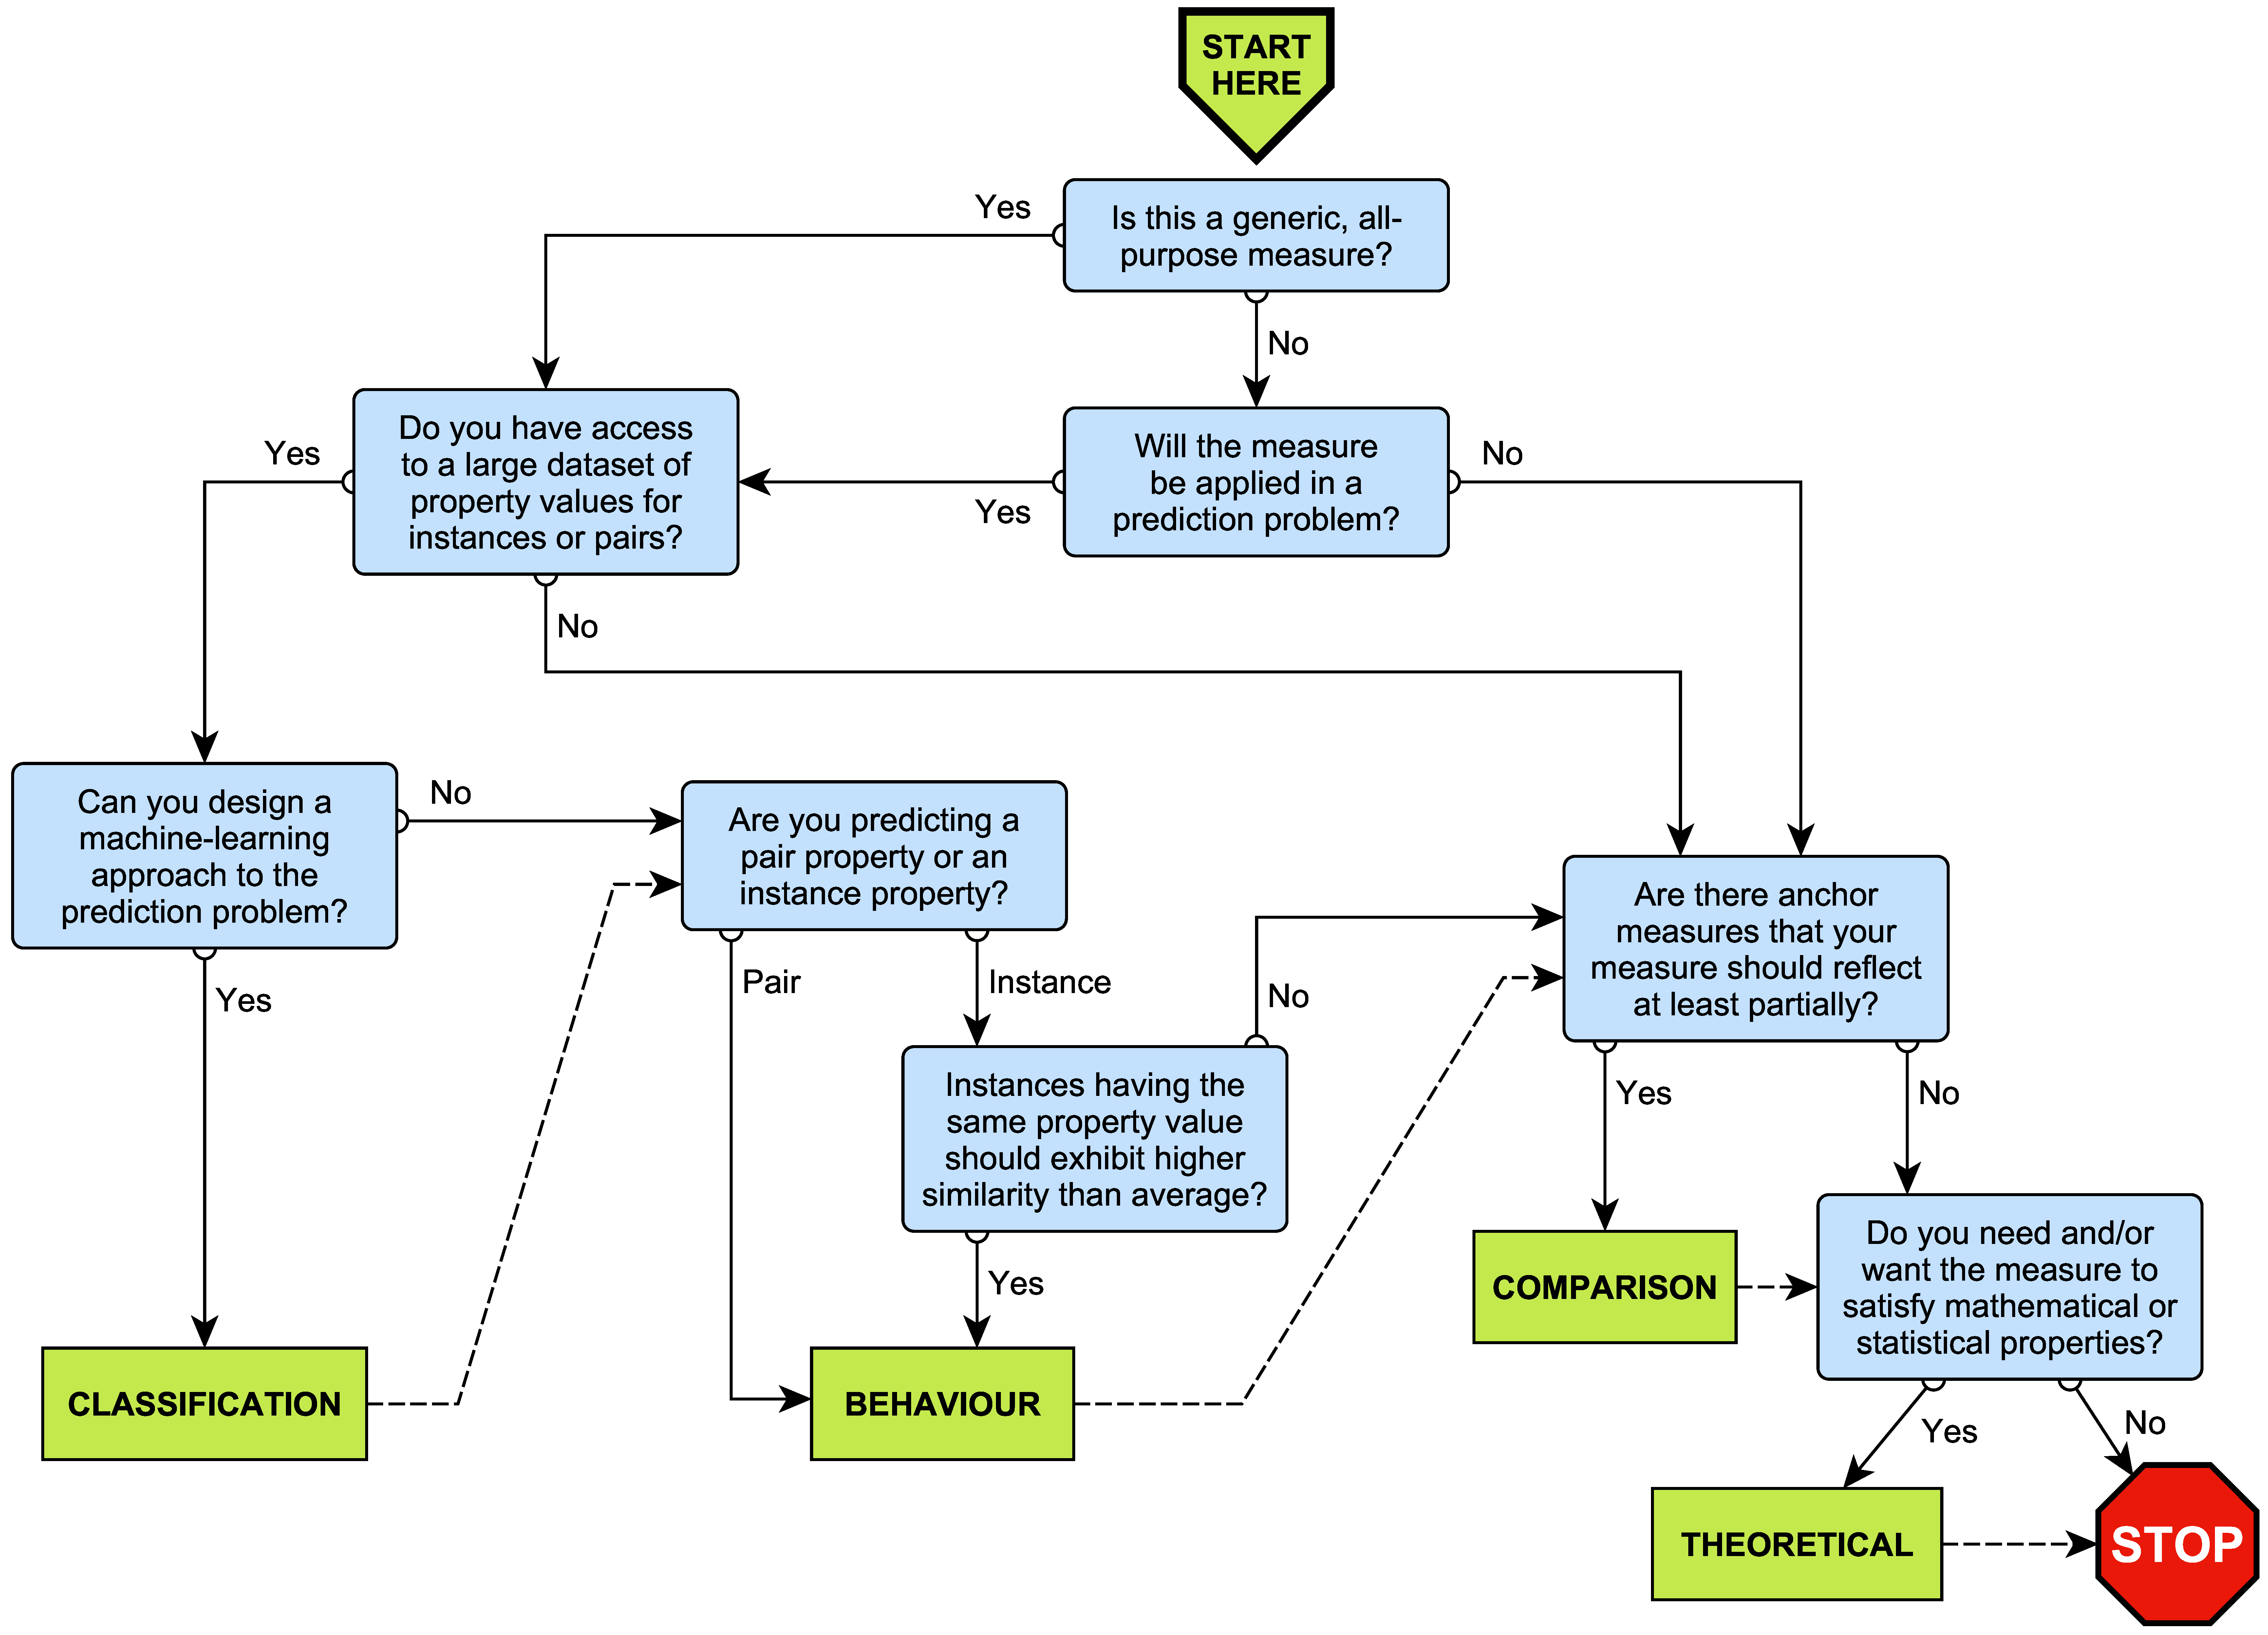
\includegraphics[width=0.8\textheight]{images/diagram.pdf}
    \end{turn}
    \caption[Pipeline to assist semantic similarity developers in the validation step]{Specific classes should be selected according to the data that the developers have access to, and to the overall goal of the measure. Questions the developers must answer are in blue rounded rectangles; strategy types are in straight green rectangles. The diagram anticipates the possibility of simultaneous validation strategies by drawing arrows from the resulting strategy types to additional questions (dashed arrows).}
    \label{fig:diagram}
\end{figure}
